\let\negmedspace\undefined
\let\negthickspace\undefined

\documentclass[journal]{IEEEtran}
\usepackage[a5paper, margin=10mm, onecolumn]{geometry}
\usepackage{tfrupee}

\setlength{\headheight}{1cm}
\setlength{\headsep}{0mm}

\usepackage{gvv-book}
\usepackage{gvv}
\usepackage{cite}
\usepackage{amsmath,amssymb,amsfonts,amsthm}
\usepackage{algorithmic}
\usepackage{graphicx}
\usepackage{textcomp}
\usepackage{xcolor}
\usepackage{txfonts}
\usepackage{listings}
\usepackage{enumitem}
\usepackage{mathtools}
\usepackage{gensymb}
\usepackage{comment}
\usepackage[breaklinks=true]{hyperref}
\usepackage{tkz-euclide}
\def\inputGnumericTable{}
\usepackage[latin1]{inputenc}
\usepackage{color}
\usepackage{array}
\usepackage{longtable}
\usepackage{calc}
\usepackage{multirow}
\usepackage{hhline}
\usepackage{ifthen}
\usepackage{lscape}
\begin{document}

\bibliographystyle{IEEEtran}
\vspace{3cm}

\title{2.3.12}
\author{EE25BTECH11009 - Anshu kumar ram}
{\let\newpage\relax\maketitle}

\renewcommand{\thefigure}{\theenumi}
\renewcommand{\thetable}{\theenumi}
\setlength{\intextsep}{10pt}
\numberwithin{equation}{enumi}
\numberwithin{figure}{enumi}
\renewcommand{\thetable}{\theenumi}

\parindent 0px
\textbf{Question:} \\
Find the angle which the line $\frac{x}{1}=\frac{y}{-1}=\frac{z}{0}$ makes with the positive direction of the Y axis.

\solution \\

   
$ Line = \myvec{0\\0\\0} + k \myvec{1\\-1\\0}$ 
\\

Hence its direction vector is

\begin{align}
\vec{v} &= \myvec{1\\-1\\0} \\
\vec{v}^T\vec{e_2} &= 
\myvec{1 & -1 & 0}\myvec{0\\1\\0}=-1 \\
\|\vec{v}\| &= 
\sqrt{\vec{v}^T\vec{v}}
=\sqrt{\myvec{1 & -1 & 0}\myvec{1\\-1\\0}}=\sqrt{2} \\
\|\vec{e_2}\| &=1 \\
\cos\theta &= 
\frac{\vec{v}^T\vec{e_2}}{\|\vec{v}\|\|\vec{e_2}\|}
=\frac{-1}{\sqrt{2}} \\
\theta &= \cos^{-1}\!\brak{-\frac{1}{\sqrt{2}}}
\end{align}

Therefore,
$
\boxed{\theta=\cos^{-1}\!\brak{-\tfrac{1}{\sqrt{2}}}\;\approx\;135\degree}
$

\begin{figure}[ht!]
\centering
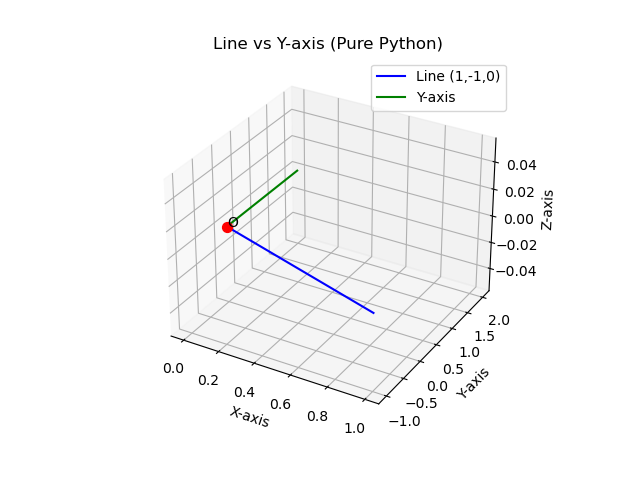
\includegraphics[width=\columnwidth, height=0.8\textheight, keepaspectratio]{figs/line.png}
\captionof{figure}{Graph}
\end{figure}

\end{document}
